\subsubsection{P2P Chord}
Die Peer-to-Peer (P2P) Chord-Architektur ist ein verteiltes Hashtabellen-System, das auf einem strukturierten Overlay-Netzwerk basiert und eine wichtige Rolle in verteilten Systemen spielt. Chord wurde erstmals 2001 von Ion Stoica, Robert Morris, David Karger, M. Frans Kaashoek und Hari Balakrishnan in ihrem wissenschaftlichen Artikel \enquote{Chord: A Scalable Peer-to-peer Lookup Service for Internet Applications} vorgestellt. Die Hauptziele der Chord-Architektur sind Skalierbarkeit, Fehlertoleranz, Lastverteilung und Dezentralisierung.
\\\\
Struktur und Funktionsweise:
\begin{itemize} 
\item \textbf{Identifier Space}: Chord definiert einen Identifier-Raum (normalerweise ein Ring) mit einem festen Wertebereich. Jeder Knoten (Peer) und jeder Schlüssel im Netzwerk erhält einen eindeutigen Identifier, der durch eine Hash-Funktion (z.B. SHA-1) erzeugt wird.
\item \textbf{Key-Node Mapping}: Jeder Schlüssel wird dem Knoten zugewiesen, der seinem Identifier am nächsten ist. Dadurch kann jeder Knoten durch Hashing des Schlüssels leicht ermitteln, welchem Knoten eine bestimmte Ressource (z.B. Datei oder Service) zugeordnet ist.
\item \textbf{Finger Tables}: Jeder Knoten im Chord-Netzwerk speichert eine sogenannte \enquote{Finger Table}, die Informationen über andere Knoten im Netzwerk enthält. Diese Tabelle ermöglicht effiziente und schnelle Routing-Operationen, da sie in jedem Schritt die Distanz zum Zielknoten mindestens halbiert. Die Finger Table enthält Verweise auf Knoten, die exponentiell weiter in der Größe entfernt sind, wodurch die Gesamtzahl der Schritte zur Lokalisierung eines Knotens logarithmisch zur Anzahl der Knoten im Netzwerk wird.
\item \textbf{Lookup-Operationen}: Wenn ein Knoten eine Anfrage nach einem bestimmten Schlüssel erhält, kann er entweder direkt die zugeordnete Ressource bereitstellen, wenn der Schlüssel diesem Knoten zugewiesen ist, oder die Anfrage entlang der Finger Table an den nächstgelegenen bekannten Knoten weiterleiten. Dieser Vorgang wird wiederholt, bis der zuständige Knoten gefunden wird. Aufgrund der Struktur der Finger Table ist die Anzahl der benötigten Schritte logarithmisch zur Anzahl der Knoten im Netzwerk.
\item Dynamik und Fehlertoleranz: Chord ist in der Lage, Knoten hinzuzufügen oder zu entfernen, ohne die Funktionsfähigkeit des gesamten Systems zu beeinträchtigen. Dazu werden die Finger Tables und die Key-Node-Zuordnungen entsprechend aktualisiert. Chord bietet auch Fehlertoleranz durch redundante Speicherung von Informationen und regelmäßige Aktualisierung der Finger Tables und Verweise zwischen Knoten.
\end{itemize} 

Es existieren zahlreiche Beispiele für Anwendungen, die sämtliche Ideen der Chord Architektur aufnehmen oder auch nur teilweise implementieren. Die folgende Aufzählung ist bei weitem nicht umfassend und soll nur einen Eindruck über die Möglichkeiten vermitteln:
\begin{itemize} 
\item Dateifreigabe: Chord kann als Basis für verteilte Dateispeicherung und -freigabe verwendet werden, wie es in Systemen wie BitTorrent und anderen P2P-Filesharing-Plattformen der Fall ist. Benutzer können Dateien hochladen und herunterladen, ohne auf zentrale Server angewiesen zu sein, wodurch die Last und Abhängigkeiten verteilt werden.
\item Distributed Domain Name System (DDNS): Chord kann zur Implementierung eines verteilten Domain Name Systems (DNS) eingesetzt werden, das die Zuordnung von Domainnamen zu IP-Adressen verwaltet. Durch die Verwendung von Chord wird das System dezentralisiert, wodurch es weniger anfällig für zentrale Angriffe oder Ausfälle ist.
\item Content Distribution Networks (CDN): Chord kann zur effizienten Verwaltung und Verteilung von Inhalten in CDNs verwendet werden. Die Knoten speichern und verteilen dabei Teile der Inhalte, um den Zugriff auf diese Ressourcen zu beschleunigen und den Verkehr auf zentralisierten Servern zu reduzieren.
\item Distributed Databases: Chord kann als Basis für verteilte Datenbanksysteme verwendet werden, bei denen die Daten und Anfragen auf mehrere Knoten verteilt werden, um die Lastverteilung zu verbessern und die Fehlertoleranz zu erhöhen.
\end{itemize}     

Die P2P Chord-Architektur ist ein bedeutender Ansatz für verteilte Systeme, da sie Skalierbarkeit, Fehlertoleranz, Dezentralisierung und Lastverteilung ermöglicht.  Die Chord-Architektur hat die Art und Weise, wie verteilte Systeme entwickelt und implementiert werden, grundlegend verändert und ermöglicht den Aufbau von effizienten und robusten dezentralisierten Anwendungen, die in der Lage sind, mit den Anforderungen moderner Internetanwendungen und der ständig wachsenden Benutzerbasis Schritt zu halten. Chords Einfluss reicht weit über den Bereich der verteilten Systeme hinaus und hat auch dazu beigetragen, die Grundlagen für die Entwicklung von Blockchain-Technologien und dezentralisierten autonomen Organisationen (DAOs) zu legen, die auf ähnlichen Prinzipien der Dezentralisierung und Konsensfindung basieren.
\\\\
Um die Funktionsweie eines Chord-Netzes zu verdeutlichen, entwickeln wir im folgenden ein Beispiel mit 16 Schlüsselplätzen. Das Beispiel zeigt wie sich in einem Chord-Netzwerk Knoten (Nodes) auf die Schlüsselplätze aufteilen.
Die Graphik~\ref{fig:chord} soll eine Idee der notwendigen Ring-Topologie des Overlay-Netzwerks geben.  

\begin{figure}[!ht]
  \centering
  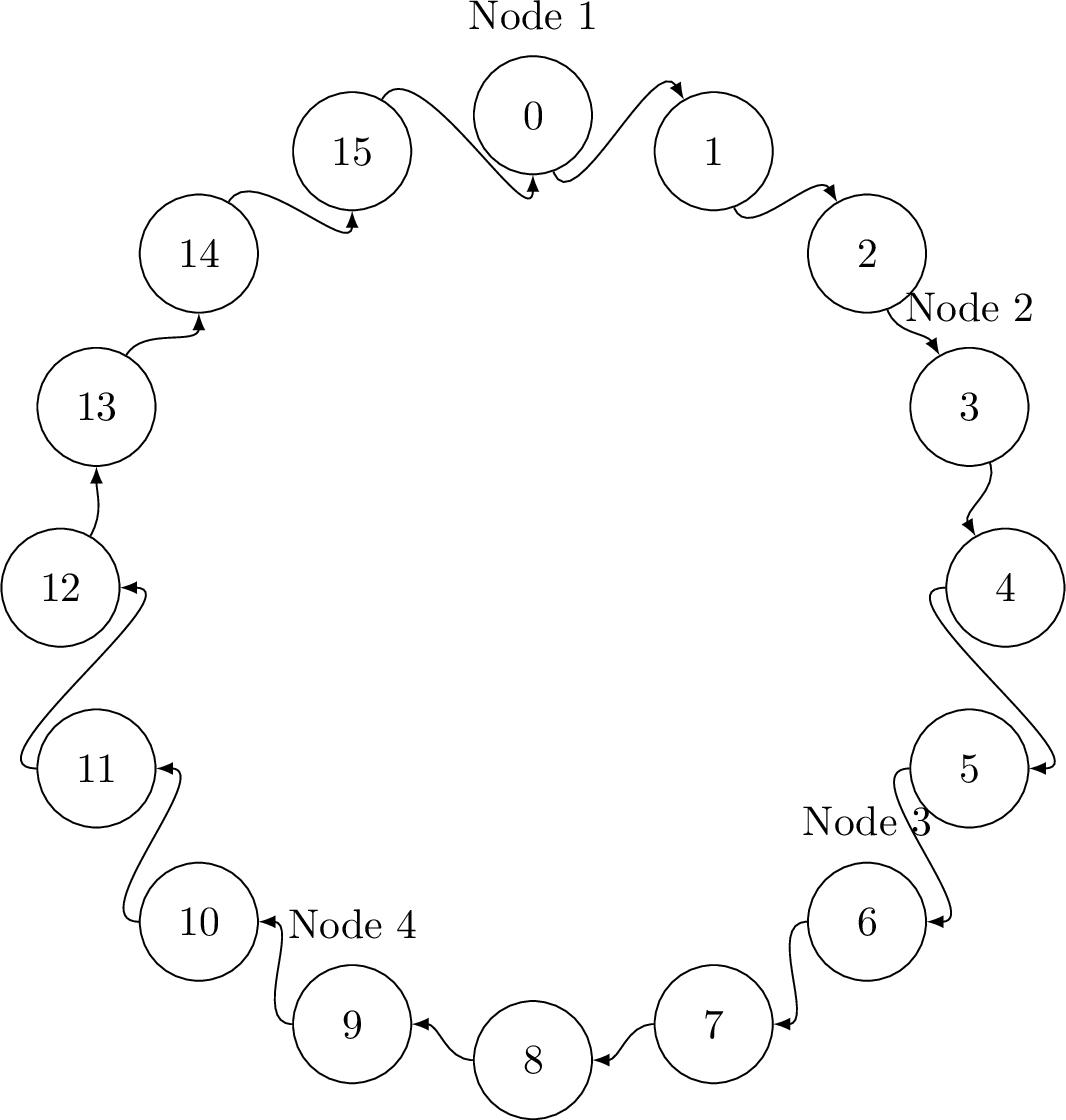
\includegraphics[width=0.45\textwidth]{fig/tex-grapics/chord.pdf.png}
  \caption{Chord Setup}
  \label{fig:chord}
\end{figure}

In diesem Beispiel sind die Knoten (Nodes) im Identifier-Raum wie folgt verteilt: Node 1: ID 0, Node 2: ID 3, Node 3: ID 6, Node 4: ID 9, Node 5: ID 13. Die Idee beim Chord Netz ist, dass der Knoten mit seiner zugeordneten ID verantwortlich ist für einen Bereich größer oder kleiner-gleich seiner eigenen ID. Dies würde für dieses Beispiel bedeuten, wenn der größer-gleich Bereich angenommen wird, dass Node 1 verantwortlich ist für die Keys 0-2, Node 2 verantwortlich für Key 3-5, Node 3 für 6-8, Node 4 für 9 -12 und Node 5 für 13-15. 

\begin{figure}[!ht]
  \centering
  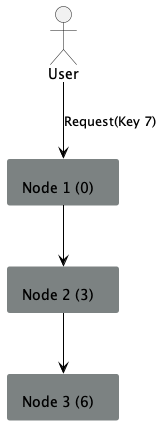
\includegraphics[width=0.15\textwidth]{fig/uml/chord.png}
  \caption{Chord Lookup Example ohne Fingertable}
  \label{fig:chord-lookup}
\end{figure}
Für das Auffinden der Nodes ohne Optimierung wie Fingertables ist nun eine lineare Suche über den Ring notwendig, der in der Graphik~\ref{fig:chord-lookup} beschrieben ist. Eine Suche (Lookup) für den Key 7 wird an dem Node 1 abgesetzt\footnote{Die Anfrage könnte auch an jeden anderen Knoten gestellt werden}. Node 1 ist nicht verantwortlich und leitet an Node 2 weiter, der sie schließlich an Node 3 weiterleitet. Node 3 ist für Key 7 zuständig und wird die angeforderte Ressource zurückgeben.
\\\\
Um den Suchaufwand zu reduzieren, kann zusätzlicher Aufwand für Strukturen betrieben werden, die wir als Fingertables bezeichnen. 
Fingertables sind ein zentraler Bestandteil der Chord-Architektur, die eine effiziente und schnelle Suche nach Schlüsseln und Knoten im Netzwerk ermöglichen. In einem Chord-Netzwerk speichert jeder Knoten eine Fingertable, die Informationen über andere Knoten im Netzwerk enthält. Die Fingertable besteht aus mehreren Einträgen, wobei jeder Eintrag auf einen \enquote{Finger} im Chord-Ring verweist. Die Funktionsweise von Fingertables kann wie folgt beschrieben werden:
\begin{itemize} 
\item Jede Fingertable hat genau $log(n)$ Einträge, wobei n die Anzahl der Knoten im Netzwerk ist.
\item Der i-te Eintrag in der Fingertable eines Knotens n verweist auf den ersten Knoten, der gleich oder nach $(n + 2^{(i-1)}) \mod 2^m$ liegt, wobei m die Anzahl der Bits für den Schlüsselraum ist (z. B. 160 für SHA-1) und i von 1 bis $log(n)$ reicht.
\item Fingertables ermöglichen eine schnelle Suche nach dem verantwortlichen Knoten für einen bestimmten Schlüssel, indem sie den Suchraum bei jedem Schritt effektiv halbieren. Dies wird erreicht, indem sie bei der Suche den nächstbesten Knoten wählen, der näher am gewünschten Schlüssel liegt.
\end{itemize} 

Damit die Fingertables wie erwartet funktionieren, muss sichergestellt werden, dass das Chord-Netzwerk  korrekt initialisiert ist, und alle Knoten müssen ihre Fingertables korrekt aufgebaut haben. Weiter müssen die Knoten im Netzwerk einvernehmliche und konsistente Informationen über die Schlüsselverteilung und die Positionen der anderen Knoten haben. Die Fingertables sollten regelmäßig aktualisiert werden, um Änderungen im Netzwerk - wie das Hinzufügen oder Entfernen von Knoten - zu berücksichtigen und sicherzustellen, dass die Routing-Informationen stets aktuell sind.

Die Verwendung ermöglicht eine effiziente Suche im Chord-Netzwerk, da sie den Suchraum bei jedem Schritt halbieren. Bei einem Lookup wird der am besten passende Knoten aus der Fingertabele ausgewählt, der näher am Ziel liegt, wodurch die Anzahl der Sprünge im Netzwerk verringert wird. Da die Fingertabele $log(n)$ Einträge hat, beträgt die maximale Anzahl der Sprünge, die benötigt werden, um einen Schlüssel zu finden, ebenfalls $log(n)$, dies auf die Hashfunktion zurückzuführen, die diese Verteilung sicherstellt. 
\\\\
Dies ist ein erheblicher Vorteil gegenüber einer naiven linearen Suche, bei der jeder Knoten einzeln überprüft werden müsste, bis der verantwortliche Knoten gefunden ist, was im schlimmsten Fall n Schritte erfordert.

\paragraph{Apache Cassandra Projekt\\\\}
Ein wichtiges Open Source Projekt, das auch der Chord Architektur basiert, ist das Apache Cassandra Projekt, welches hier kurz vorgestellt werden soll. Apache Cassandra ist ein verteiltes, hochverfügbares und skalierbares NoSQL-Datenbanksystem, das sich von der Chord-Architektur inspirieren ließ. Im Gegensatz zum klassischen Chord-Netzwerk hat Cassandra jedoch einige Anpassungen und Erweiterungen vorgenommen, um den Anforderungen moderner verteilter Datenbanksysteme gerecht zu werden. Durch dieses Projekt sollen einige Techniken eingeführt werden, die in der späteren Diskussion nochmal aufgenommen werden sollen. Weiter soll die Ausführung aufzeigen, wie bestehende Ideen über die Zeit Anpassungen und Optimierungen erfahren.

Einige der Anpassungen, die Apache Cassandra im Vergleich zur Chord-Architektur vorgenommen hat, sind:
\begin{itemize} 
\item Partitionierungsstrategie: In Cassandra werden Daten über mehrere Knoten (Nodes) verteilt, indem sie auf Basis eines Partitionsschlüssels, der aus den Eingabedaten extrahiert wird, partitioniert werden. Die Verantwortlichkeit für die Daten wird anhand eines konsistenten Hashing-Algorithmus, ähnlich wie bei Chord, bestimmt.

Die Hauptidee hinter Partitionierungsstrategien besteht darin, den Datenraum in kleinere Partitionen aufzuteilen und diese auf die verschiedenen Knoten im Cluster zu verteilen. Dadurch wird die Last gleichmäßiger auf die Knoten verteilt, und es wird verhindert, dass einige Knoten überlastet werden, während andere Knoten ungenutzt bleiben.

Cassandra verwendet einen Partitionsschlüssel, um den Platz einer Zeile innerhalb einer Tabelle zu bestimmen. Dieser Partitionsschlüssel wird durch einen Partitionierer, wie den Murmur3Partitioner, in einen Token-Wert konvertiert. Der Token-Wert wird dann verwendet, um den verantwortlichen Knoten für diese Partition zu bestimmen.

Sharding ist eine Partitionierungsstrategie, die in verteilten Datenbanksystemen verwendet wird, um Daten auf verschiedene Knoten oder Server aufzuteilen. So wird der gesamte Datensatz in kleinere, handhabbare Teile (Shards) aufgeteilt, wobei jeder Shard auf einem separaten Knoten oder Server gespeichert wird. Sharding kann auf verschiedene Arten implementiert werden, wie z.B.:
\begin{itemize} 
\item Range-based Sharding: Die Daten werden basierend auf einem bestimmten Wertebereich aufgeteilt. Zum Beispiel könnten Kundeninformationen basierend auf der Kunden-ID in unterschiedliche Shards aufgeteilt werden, wobei ein Shard Kunden-IDs von 1 bis 10.000, ein anderer Shard Kunden-IDs von 10.001 bis 20.000 usw. enthält.
\item Hash-based Sharding: Die Daten werden basierend auf einem Hash-Wert aufgeteilt, der aus dem Partitionsschlüssel berechnet wird. In diesem Fall wird der Hash-Wert verwendet, um die Daten gleichmäßig auf die verfügbaren Knoten zu verteilen.
\end{itemize}  
\item Replikationsstrategie: Um Datenverlust zu verhindern und hohe Verfügbarkeit zu gewährleisten, repliziert Cassandra Daten über mehrere Knoten hinweg. Die Anzahl der Replikationen und die Replikationsstrategie können konfiguriert werden. Im Gegensatz zum Chord-Netzwerk, das nur die direkten Nachfolgerknoten für die Replikation verwendet, unterstützt Cassandra verschiedene Replikationsstrategien wie SimpleStrategy und NetworkTopologyStrategy, um eine bessere Kontrolle über die Replikationslogik zu ermöglichen.
\item Datenmodell: Cassandra verwendet ein spaltenorientiertes Datenmodell, das sich von traditionellen relationalen Datenbanken unterscheidet. Das Datenmodell basiert auf einer Tabelle mit einer oder mehreren Partitionen, die wiederum aus einer oder mehreren Zeilen bestehen. Jede Zeile enthält einen eindeutigen Schlüssel und einen oder mehrere Spalten, die die Daten speichern.
\item Gossip-Protokoll: Im Gegensatz zur Chord-Architektur, die Fingertables für das Routing verwendet, verwendet Cassandra ein Gossip-Protokoll für die Kommunikation und den Informationsaustausch zwischen den Knoten. Das Gossip-Protokoll ermöglicht es Knoten, regelmäßig Informationen über ihren Status, ihre Last und die Topologie des Netzwerks auszutauschen.
\item Lese- und Schreibkonsistenz: Cassandra bietet die Möglichkeit, die Konsistenz von Lese- und Schreibvorgängen je nach Anforderungen der Anwendung anzupassen. Die Konsistenz kann auf unterschiedlichen Ebenen gewählt werden, von \enquote{One} (nur ein Knoten muss den Vorgang bestätigen) bis \enquote{All} (alle Replikationsknoten müssen den Vorgang bestätigen). Dies ermöglicht eine bessere Kontrolle über die Trade-offs zwischen Konsistenz, Verfügbarkeit und Performance.
\item Hinted Handoff: Cassandra verwendet ein Mechanismus namens \enquote{Hinted Handoff}, um vorübergehend ausgefallene Knoten zu behandeln. Wenn ein Knoten nicht verfügbar ist, um eine Schreiboperation durchzuführen, speichert ein anderer Knoten einen \enquote{Hint} und stellt die Daten dem ausgefallenen Knoten zur Verfügung, sobald dieser wieder online ist. Dieses Verfahren erhöht die Verfügbarkeit und Fehlertoleranz des Systems.
\item Repair und Anti-Entropy: Im Gegensatz zur Chord-Architektur verfügt Cassandra über Anti-Entropy- und Repair-Mechanismen, um Inkonsistenzen zwischen Replikationsknoten zu erkennen und zu beheben. Cassandra verwendet Merkle Trees, um Unterschiede zwischen Replikationen effizient zu erkennen und bei Bedarf Daten synchronisieren.
\end{itemize}
\paragraph{Anti-Entropy (kurz)\\\\}
Anti-Entropy ist ein Mechanismus in verteilten Systemen, der dazu dient, die Konsistenz und Stabilität von Daten über mehrere Knoten (Nodes) hinweg sicherzustellen. In einem verteilten System arbeiten mehrere unabhängige Knoten zusammen, um eine gemeinsame Aufgabe zu erfüllen, wie zum Beispiel die Speicherung und Verwaltung von Daten. Diese Knoten können jedoch aufgrund von Netzwerkverzögerungen, Fehlern oder Abstürzen inkonsistente Daten enthalten. Diese Verfahren werden in einem späteren Kapitel nochmals genauer betrachtet. 
\\\\
Anti-Entropy-Prozesse sorgen dafür, dass die Daten auf den verschiedenen Knoten synchronisiert und konsistent bleiben. Sie verwenden Replikations- und Synchronisationsverfahren, um sicherzustellen, dass alle Knoten dieselben Daten enthalten.

\label{Woche06}
